\section{Performance of Classical Computers}

For the optimization of the Pyomo model, the Pyomo library runs a standard solver.
It formulates the problem in the mathematical modeling language AMPL
and calls a solver to optimize it.
The solver returns the solution, which is then read by Pyomo.
\cite{PyomoAMPL}

The solver that is used in this paper is called Couenne and was built by COIN-OR.
Couenne is short for ''Convex Over and Under ENvelopes for Nonlinear Estimation''.
It can find global minima of nonconvex MINLPs like the one that is formulated above.
It is a branch and bound algorithm and utilizes linearization, bound reduction, and branching methods.
\cite{CoinorHome,CouenneRepo}

The optimizations are performed on the Excess Cluster of the HLRS, Stuttgart.
\cite{ExcessHLRS,HLRS}

The optimization of the problem is of high time complexity.
In the beginning, with small inputs, it takes little time.
As listed in table \ref{table:validation.classical.performance}, the optimization of $4$ power plants with $2$ units of time takes about $0.5$ seconds.
But as the input size grows, the time needed by the solver grows exponentially.
When the input size is doubled --- $4$ plants over $4$ units of time --- the optimization takes about $3.5$ seconds.
After adding another $2$ units of time, the optimization takes $15.5$ seconds.

As the number of inputs grows large, the optimization grows even faster than exponentially.
With a worst-case projection of the first $4$ data points, the time needed for optimization should multiply by $7$ with every additional $2$ units of time.
That means that the optimization of $4$ power plants over $14$ units of time should take about $0.5 \cdot 7^6 \approx 58,824$ seconds.
But the data shows that it took about $311,144.9$ seconds.

\begin{table}[ht]
  \centering
  \begin{tabular}{| r | r | r | r |}
  \hline 
  Number of Loads & Objective function & Time (in seconds) & Time (in hours) \\ 
  \hline \hline 
  2 & 116037.074 & 0.517 & 0.000 \\ \hline 
  4 & 224372.794 & 3.617 & 0.001 \\ \hline 
  6 & 317725.099 & 15.582 & 0.004 \\ \hline 
  8 & 405214.877 & 107.714 & 0.030 \\ \hline 
  10 & 486041.406 & 1218.918 & 0.339 \\ \hline 
  12 & 560470.679 & 17292.102 & 4.803 \\ \hline 
  14 & 625146.685 & 311144.864 & 86.429 \\ \hline 
\end{tabular}

  \caption{Results of classical optimization with four power plants.}
  \label{table:validation.classical.performance}
\end{table}

The diagram \ref{figure:validation.classical.performance} highlights the exponential nature of the optimization of the problem.
It shows the time needed for optimization dependent on the input size --- the number of units of time.

\begin{figure}[ht]
  \centering
  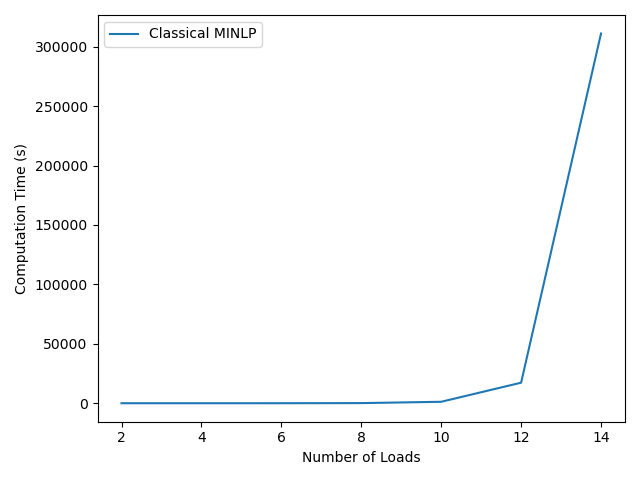
\includegraphics[width=0.75 \textwidth]{04_Validation/performance_classical_p4.png}
  \caption{Time complexity of classical optimization with four power plants.}
  \label{figure:validation.classical.performance}
\end{figure}
